\documentclass[10pt,final,journal]{IEEEtran}
\usepackage{amsfonts}
\usepackage{amssymb}
\usepackage{graphicx}
\usepackage{siunitx}
\usepackage[usenames, dvipsnames]{color}

\title{Feasibility of Harvesting Power To Run A Domestic Water Meter Using Streaming Cell Technology}

\author{Mark~H.~Jones, and Prof.~Jonathan~Scott}

\begin{document}
    \maketitle

    \begin{abstract}
        We investigate the possibility of using streaming cells as a means of harvesting energy from a town water supply.
        We verify streaming cell measurements found in the literature and extend those measurements over a wider range of dimensions.
        We measure the electrical power developed from ten streaming cells over a range of pressure differentials using town water.
        We estimate the amount of energy required to operate a simple data logger and transmitter.
        We estimate the amount of energy available from a typical domestic household based on water usage data.
        Finally, we calculate the dimensions required to build a streaming cell harvester large enough to enable domestic water consumption logging and transmission.
    \end{abstract}

    \section{Introduction}
    Domestic and commercial water metering is becoming increasingly important throughout the world.
    Having a cheap and reliable way to retrieve metering information is an important consideration for utility companies.
    There are two methods available to water utility companies when recording the volume of water delivered to consumers.
    \begin{enumerate}
        \item \emph{Mechanical readout:}
            Involves a meter-reader visually sighting the meter's readout from time to time.
            Generally the reading frequency is kept to a minimum and estimate readings are made in the interim.
        \item \emph{Electronic telemetry:}
            Wireless data transmission is increasingly becoming used as a method of metering data recovery.
            Due to the location of water metering, electrical power must be provided by long life batteries.
            These batteries are usually non-rechargeable and therefore must be replaced once exhausted.
        \end{enumerate}
    {\color{blue}[Suggested adding references to the above items. Not really sure what I would be adding - a specific example would be good]}
    The methods previously mentioned are costly to the utility as they require periodic human intervention.
    Even in the case of wireless data transmission, batteries
    The possibility of harvesting energy at the meter will allow periodic data transmission with less maintenance.
    Removing batteries from electrical meters also reduces unwanted electrical waste.

    Streaming cells provide a way of converting fluid pressure/flow into electrical voltage/current.
    Charged surfaces in contact with ionic solutions attract counter-ions\footnote{The terms counter-ion and co-ion refer to ions of opposite and like charge relative to the polarity of the solid surface respectively.} while repelling co-ions so as to form a charged layer.~\cite{Stein2004}
    This charged layer is termed the double layer and is the key mechanism that enables streaming cell energy conversion.

    A double layer can be broken into two sub-layers; the Stern and diffuse layers.
    The Stern layer is comprised of immobilised ions situated very close the charged solid surface.~\cite{Salieb-Beugelaar2009}
    The diffuse layer is formed by the ions attracted to the surface, but not so strongly as to be immobile.

    A streaming cell makes use of ions at the interface by forcing them through one or more narrow channels.
    The channels can be formed from porous materials or created individually by various fabrication methods, e.g. chemical etching.
    By immersing a channel in an electrolyte solution, double layers line the interior to the channel.
    The thickness of the double layer is represented by the Debye length ($l_{D}$) and is controlled the ionic concentration of the liquid.~\cite{Israelachvili2011}
    When the dimensions of a channel become small enough the double layers begin to overlap and co-ions are repelled from the channel.

    Counter-ions within a streaming cell are collected by applying a pressure gradient across the channel/cell.
    Pressure forces the liquid through the channel (from which co-ions have been removed) creating a streaming current.
    It is the streaming current that raises the voltage (streaming potential) across the cell as the ions are pumped through it.

    Streaming currents have been heavily investigated as a means of generating electrical energy from pressure gradients.~\cite{Chang2009,Daiguji2006,Daiguji2004b,Davidson2008a,Davidson2008,CherngHon2012,Jiao2014,Lu2006,Olthuis2005,Osterle1964,Pennathur2007,Ren2008a,VanderHeyden2006,Heyden2007,Xie2008,Yang2003}
    % It is expected that a channel height equal to twice the Debye length leads to maximum energy conversion efficiency.~\cite{Daiguji2004b}
    Theoretical predictions of the efficiency of standard micro/nano-fluidic channels are 2\% for pure water and 7\% for sodium chloride.~\cite{VanderHeyden2006}
    Experimental results show conversion efficiencies in the range of:
    \begin{itemize}
        \item 0.01\% by forcing water through porous glass with pore sizes from 10\thinspace--\SI{16}{\micro\metre}.~\cite{Yang2003}
        \item 0.8\% by forcing pure water through a ceramic rod populated with \SI{6}{\micro\metre} pores.~\cite{Yang2004}
        \item 3\% by forcing sodium chloride solution through a \SI{75}{\nano\metre} by \SI{50}{\micro\metre} silica channel.~\cite{Heyden2007}
        \item 0.77\% by forcing sodium chloride through a \SI{200}{\nano\metre} pore in an alumina membrane.~\cite{Lu2006}
        \item 5\% by forcing sodium chloride solution through a \SI{0.5}{\nano\metre} cylindrical pore in polyethylene terephalate foil.~\cite{Xie2008}
    \end{itemize}

    It is clear from the literature that there is significant progress to be made with respect to increasing the conversion efficiency.
    Techniques to induce hydrodynamic slip at the fluid-solid interface are predicted to increase this efficiency to 30-40\%.~\cite{Davidson2008a, Ren2008a}
    However, experimental results utilising slip enhanced channels have not yet been reported in the literature.
    This type of enhancement would overcome the no-slip boundary condition at the solid-liquid interface of the cavity - where ionic concentration is at its highest.
    In~\cite{Joly2006} it is suggested that a polarised hydrophobic surface would strongly enhance electro-osmotic effects and therefore further increase conversion efficiency.
    Hydrophobic channels have not been considered due to the exotic materials required to build them.

    We address the question of whether it is feasible to build a harvester using readily available materials.
    Such a harvester must produce enough energy to operate a microprocessor and radio communication device.
    It must collect all of its energy from a domestic water supply and be reliable.

    The remainder of this work is presented as follows.
    In section \ref{sect:streamingCell} we build and measure a simple streaming potential cell.
    We confirm the relationship between pressure and applied pressure and investigate the effect of channel height.
    In section \ref{sect:waterConsumption} we estimate a typical domestic water usage profile.
    This consumption profile will be used as the basis for estimating the amount of energy available to the harvester.
    Section \ref{sect:powerRequirements} determines the amount of energy an electronic meter would need to be useful.
    Following on this, section \ref{sect:harvesterSize} presents the required dimensions a usable harvester would need.
    Finally we discuss the feasibility of using in the conclusion.

    \section{Readily Attainable Streaming Cell Power} \label{sect:streamingCell}
    In~\cite{Gu2000}, the authors employ a relatively simple parallel plate design to create a streaming cell.
    Sandwiching plastic shims between plates of glass provided a simple way to control channel height.
    Using that method, the authors of~\cite{Gu2000} fabricated three cells with channel heights of \SI{50}{\micro\metre}, \SI{100}{\micro\metre} and \SI{150}{\micro\metre}.
    Each of the channels were \SI{3}{\centi\metre} long and had a inner width of \SI{1}{\centi\metre}.

    \begin{figure}
        \begin{center}
        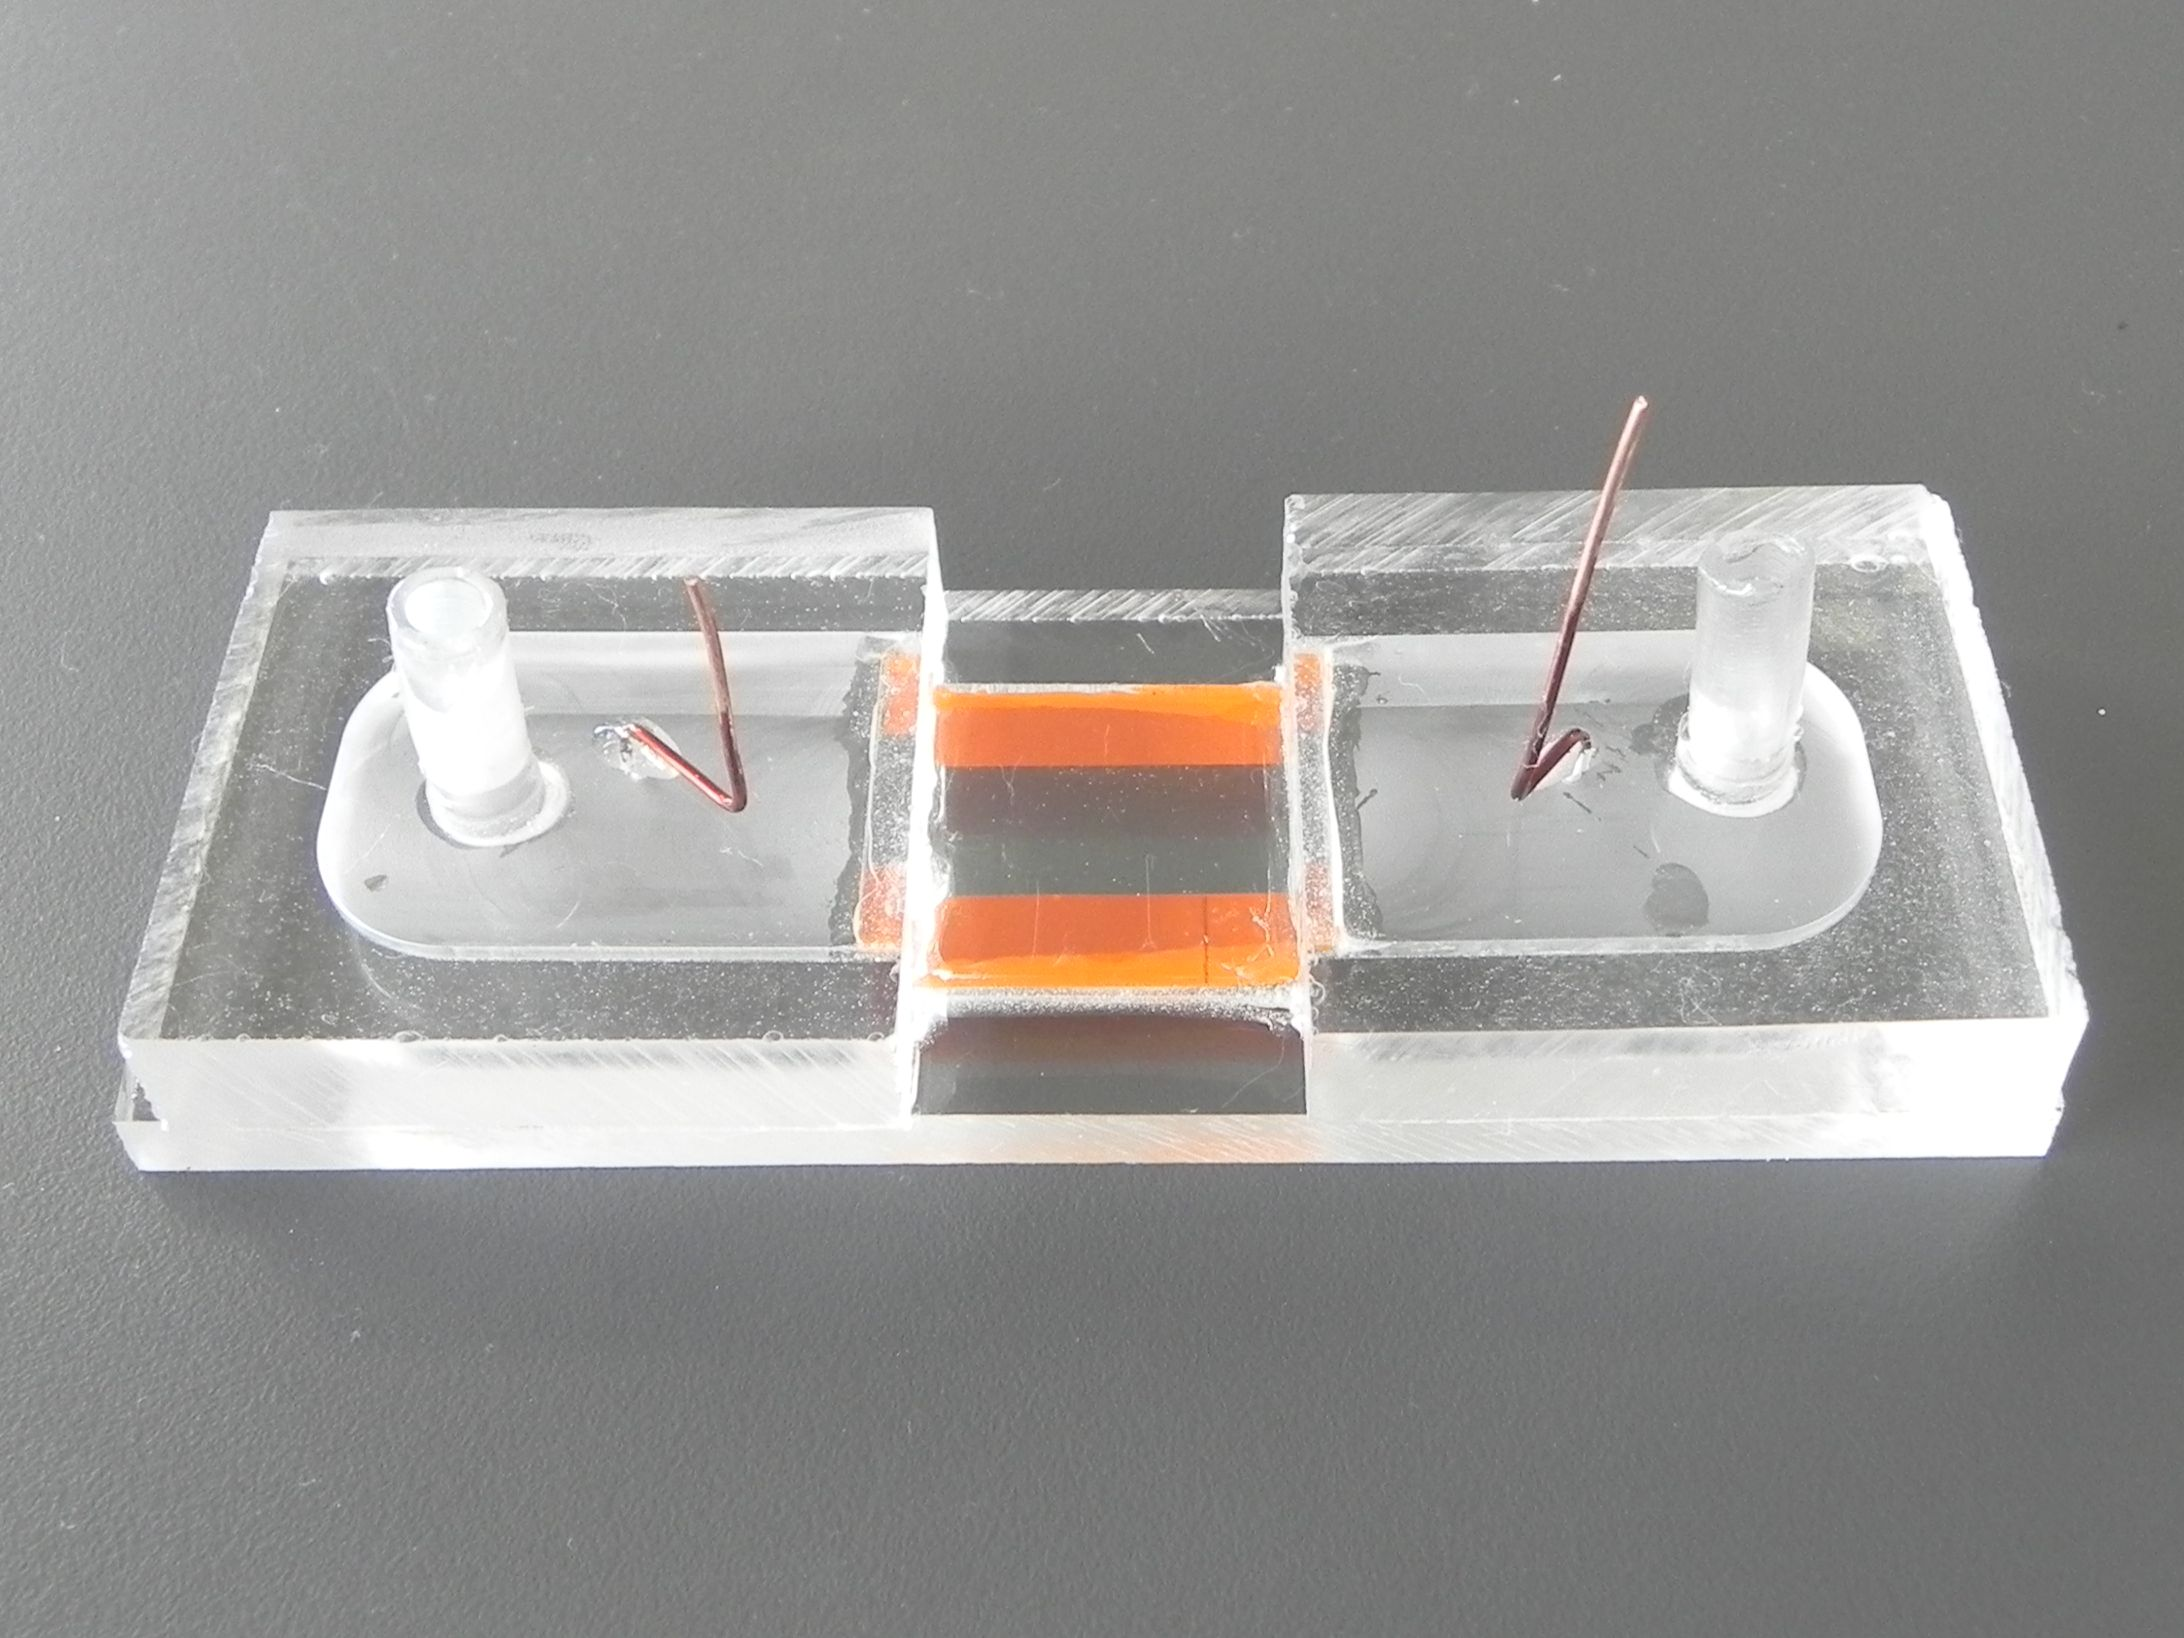
\includegraphics[width=\linewidth]{Photo_streamingPotential_Assembly_Step3.JPG}
        \end{center}
        \caption{One of ten constructed streaming cells mounted in an acrylic holder. Copper wires have been epoxied into each side to provide a means of measuring the developed potential across the cell. The shim is visible as the two orange strips at each side of the cell.}
        \label{fig:cell}
    \end{figure}

    We replicate the fabrication method and approximate dimensions of \cite{Gu2000} to produce ten streaming cell channels.
    The internal dimensions of which are \SI{3}{\centi\metre} long, \SI{1}{\centi\metre} wide and heights in the range of \SI{25}{\micro\metre} to \SI{250}{\micro\metre}.
    These dimensions are directly comparable to those of \cite{Gu2000}, where the length and width are the same but the heights span a wider range.
    The channels themselves are made from glass microscope slides (Sail Brand - JIA 7101WT) which are sectioned into halves.
    Plastic shims (Garlock Colorplast) are epoxied (Selleys Araldite Ultra Clear Resin) between slide halves to create the channels.
    The dimensions at each end of each channel have been measured under a microscope to determine the actual channel height.

    Each channel is epoxied between two acrylic reservoirs and a base plate.
    This provides a rigid structure under pressure and provides connection of wires and hoses.
    Copper wires and silicon hoses are inserted into each reservoir to facilitate streaming potential measurement and f:w

    A photo of one of the cells is shown in Fig. \ref{fig:cell}.


    \begin{tabular}{|c|c|c|} \hline
    Microscope slides & Sail Brand & JIA 7101WT - 26 x 76mm\tabularnewline \hline
    Shims & Garlock & Colorplast - 50$\,\mu$m, 80$\,\mu$m, 120$\,\mu$m and 250$\,\mu$m\tabularnewline \hline
    Epoxy & Selleys & Araldite - Ultra Clear Resin\tabularnewline \hline
    Pressure Sensor & Honeywell & 24PC15SMT - 0 -- $\pm$15 PSI\tabularnewline \hline
    \end{tabular}


    \section{Estimation of Typical Household Water Consumption}:
    \label{sect:waterConsumption}
    \section{Estimation of Power Requirements}
    \label{sect:powerRequirements}
    \section{Estimation of Streaming Cell Harvester}
    \label{sect:harvesterSize}
    \section{Conclusion}
    \bibliographystyle{plain}
    \bibliography{library}

\end{document}
